\usepgfplotslibrary{polar};

\chapter{Calculus with Polar Coordinates}

We've been working in Cartesian coordinates, which are rectangular, with $x$ representing the horizontal position and $y$ representing the vertical position. Another way to represent a position in $2D$ space is with \textbf{polar coordinates}\index{polar coordinates}. In this coordinate system, the first number and independent variable is $\Theta$ and represents the degrees of rotation from the the $x$ axis. The second number is $r$ and represents how far the point is from the origin (see figure \ref{polarex}). 

\begin{figure}[htbp]
\centering
    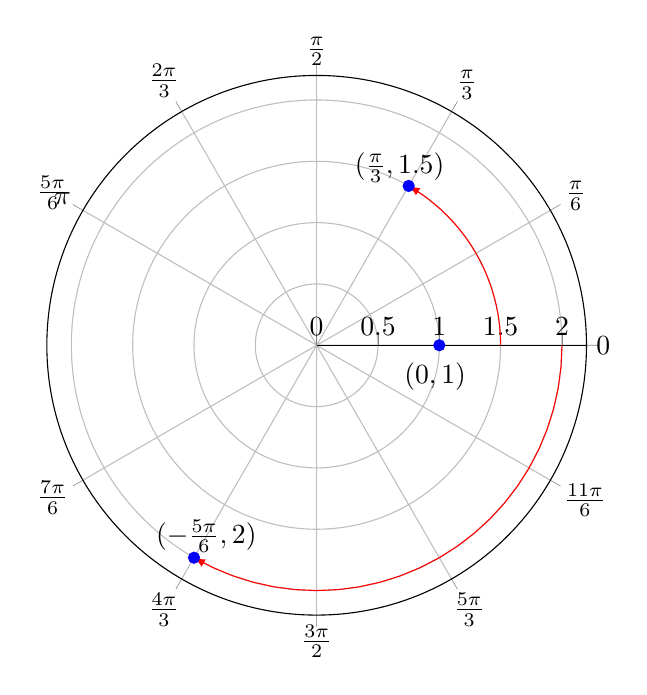
\begin{tikzpicture}
	\begin{polaraxis}[xtick = {0,0,deg((pi)/6),deg((2*pi)/6),deg((3*pi)/6),deg(4*pi)/6,deg((5*pi)/6), deg((5*pi)/6), deg((7*pi)/6), deg((8*pi)/6), deg((9*pi)/6), deg((10*pi)/6), deg((11*pi)/6)},
  xticklabels={,0,$\frac{\pi}{6}$,$\frac{\pi}{3}$,$\frac{\pi}{2}$,$\frac{2\pi}{3}$, $\frac{5\pi}{6}$, $\pi$,$\frac{7\pi}{6}$, $\frac{4\pi}{3}$, $\frac{3\pi}{2}$, $\frac{5\pi}{3}$, $\frac{11\pi}{6}$}]
        \addplot[blue, only marks]coordinates {(0,1) (60, 1.5) (240, 2)};
        \addplot[red, domain = 0:60]{1.5};
        \draw[red, -latex](58, 1.5)--(60,1.5);
        \node[] at (65, 1.6) {$(\frac{\pi}{3}, 1.5)$};
        \node[] at (-15, 1) {$(0, 1)$};
        \addplot[red, domain = -120:0]{2};
        \draw[red, -latex](-118, 2) -- (-120,2);
        \node[] at (-120, 1.8) {$(-\frac{5\pi}{6}, 2)$};
        \end{polaraxis}
    \end{tikzpicture}
    \label{polarex}
    \caption{Polar coordinates give a degree of rotation, $\Theta$, and a distance from the origin, $r$}
    \end{figure}

\section{Derivatives of Polar Functions}
Consider the cardioid $r = 2 + \sin{\Theta}$ (see figure \ref{cardioid}). What is the slope of the line tangent to the curve at $\Theta = \frac{\pi}{2}$? From a visual inspection, we can guess that the slope of the tangent line is zero. Let's prove this mathematically:

First, recall that to convert polar coordinates to Cartesian coordinates, we can use the trigonometric identities:
$$x = r\cos{\Theta}$$
$$y = r\sin{\Theta}$$

So we can write the parametric equation:
$$x = \left[2 + \sin{\Theta} \right]\cos{\Theta}$$
$$y = \left[ 2 + \sin{\Theta} \right]\sin{\Theta}$$

Recall from parametric equations that we can use implicit differentiation to find $\frac{dy}{dx}$:
$$\frac{dy}{dx} = \frac{\frac{dy}{d\Theta}}{\frac{dx}{d\Theta}}$$

And so we can find $\frac{dy}{dx}$ for this cardioid:
$$\frac{dy}{dx} = \frac{\frac{d}{d\Theta} \left(2\cos{\Theta} + \sin{Theta}\cos{Theta} \right)}{\frac{d}{d\Theta} \left(2\sin{\Theta} + \sin^2{\Theta} \right)}$$

\begin{figure}
\centering
    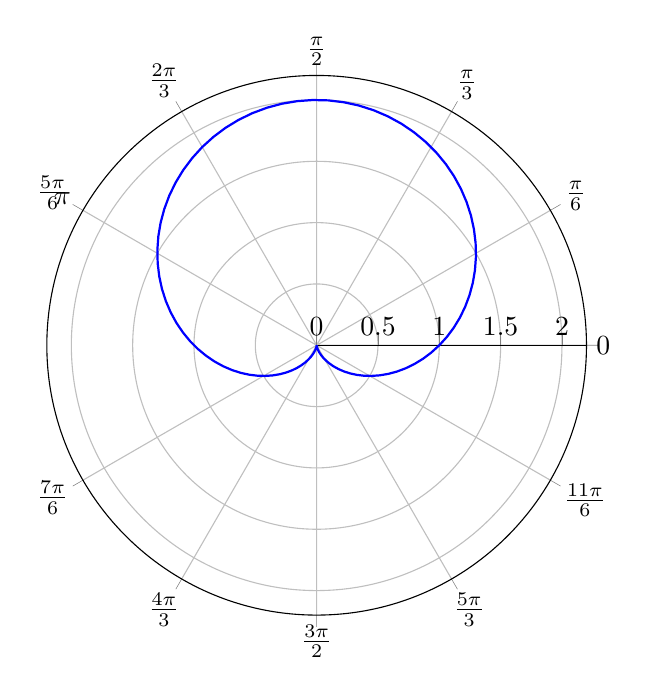
\begin{tikzpicture}
	\begin{polaraxis}[xtick = {0,0,deg((pi)/6),deg((2*pi)/6),deg((3*pi)/6),deg(4*pi)/6,deg((5*pi)/6), deg((5*pi)/6), deg((7*pi)/6), deg((8*pi)/6), deg((9*pi)/6), deg((10*pi)/6), deg((11*pi)/6)},
  xticklabels={,0,$\frac{\pi}{6}$,$\frac{\pi}{3}$,$\frac{\pi}{2}$,$\frac{2\pi}{3}$, $\frac{5\pi}{6}$, $\pi$,$\frac{7\pi}{6}$, $\frac{4\pi}{3}$, $\frac{3\pi}{2}$, $\frac{5\pi}{3}$, $\frac{11\pi}{6}$}]
        \addplot[blue, thick, domain = 0:360, samples = 100]{1 + sin(x)};
        \end{polaraxis}
    \end{tikzpicture}
    \label{cardioid}
    \caption{$r = 2 + \sin{\Theta}$}
    \end{figure}


\begin{Exercise}[label = polar1]
[This problem was originally presented as a no-calculator, multiple-choice 
question on the 2012 AP Calculus BC exam.] What is the slope of the line 
tangent to the polar curve $r = 1 + 2\sin{\Theta}$ at $\Theta = 0$?
\end{Exercise}

\begin{Answer}[ref = polar1]
Recall that for a polar function, $\frac{dy}{dx} = \frac{\frac{dr}{d\Theta}
\sin{\Theta} + r\cos{\Theta}}{\frac{dr}{d\Theta}\cos{\Theta} - r\sin{\Theta}}$. 
At $\Theta = 0$, $r = 1 + 2\sin{0} = 1$ and $\frac{dr}{d\Theta} = 2\cos{0} = 
2$. Substituting, we find that $\frac{dy}{dx} = \frac{2\sin{0} + 1\cos{0}}{2
\cos{0} - 1\sin{0}} = \frac{0 + 1}{2 - 0} = \frac{1}{2}$. 
\end{Answer}

\begin{Exercise}[label = polar2]
The figure below shows the graphs of polar curves $r = 2\cos{3\Theta}$ and $r = 2$. What is the sum of the areas of the shaded regions?	[fix me graph]
\end{Exercise}

\begin{Answer}[ref = polar2]
We know the area of the circle is $\pi r^2 = \pi(2)^2 = 4\pi$. To find the area of the shaded regions, we need to subtract the area of the trefoil from the area of the circle. The area of the trefoil is given by $\frac{1}{2} \int_0^{\pi} \left[2 \cos{3\Theta} \right]^2\,d\Theta =$
\end{Answer}